% https://github.com/darwiin/yaac-another-awesome-cv
%
% Author:
% Christophe Roger
%
% Template license:
% CC BY-SA 4.0 (https://creativecommons.org/licenses/by-sa/4.0/)

%Section compétences

\sectionTitle{Publications}{\faBook}
\begin{minipage}[t]{0.75\textwidth}
\begin{itemize}
    \item \textbf{ Xian, Y.}, Karki, C.B., Silva, S.M., Li, L., Xiao, C. (2019) "The Roles of Electrostatic Interactions in Capsid Assembly Mechanisms of Giant Viruses." Int. J. Mol. Sci. 20, 1876. (Cover of the journal)
    
    \item \textbf{ Xian, Y.}, Silva, S.M., Karki, C.B., Li, L. (2019) "Structural operation tool: a tool to study protein-protein interactions." (To be submitted)
    
    \item \textbf{Xian, Y.}, Moreno, B., Chacon, M.C, Bolotaulo, D. M., and Xiao, C. (2019). " An Novel Integrase From the Virophage, Mavirus, and its Mechanism of Host Genome Integration." (Under revision)
    
    \item \textbf{Xian, Y.}, Karki, C., Li, L., and Xiao, C. (2019). "A Common Scheme of Capsid Assembly among Giant Viruses: Long-range Electrostatic Interactions Guide the Assembly of Capsid Proteins." (Under revision)

    \item Karki,C., \textbf{Xian, Y.}, David,V.O., Sun,J., Li,L. (2019)."Effects of pH on the complex of CFP-10/ESAT-6: Van der Waals energy compensates the electrostatic energies."  (Under revision)
    
    \item Karki,C., \textbf{Xian, Y.}, David,V.O., Sun,J., Li,L. (2019). "A computational model of Esat6 complex in membrane." (Under revision)

    \item Martin, R. M., Moniruzzaman, M., Mucci N. C., Willis, A., Woodhouse, J. N.,\textbf{ Xian Y.}, Xiao, C., Brussaard, C. P. D., Wilhelm, S. W. (2018). "Cylindrospermopsis raciborskii Virus and host: Genomic characterization and ecological relevance: Cylindrospermopsis raciborskii Virus genome." Environ Microbiol.
    

\end{itemize}
\end{minipage}
\begin{minipage}[t]{.3\textwidth}
    \centering
    \textbf{Journal Cover:}\\
    \href{https://www.mdpi.com/1422-0067/20/8}{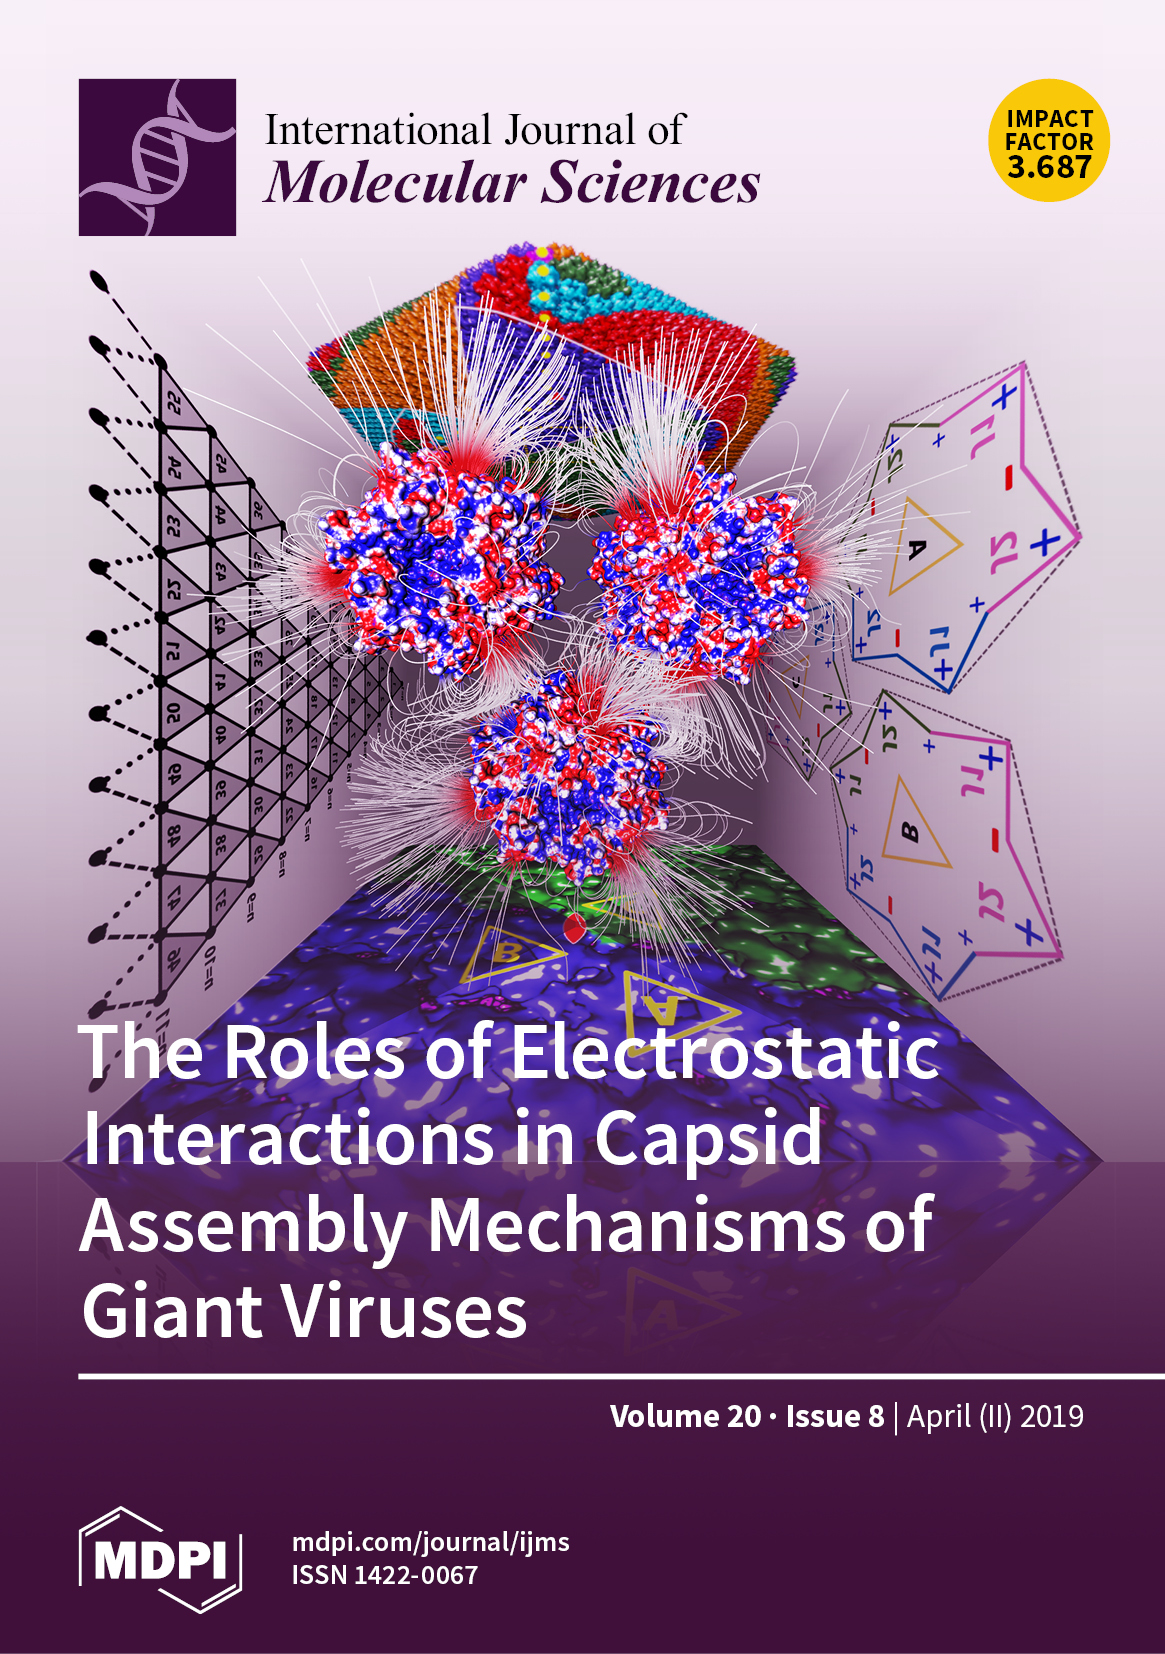
\includegraphics[width=0.7\textwidth]{IJMS-Cover.jpg}}

    Int. J. Mol. Sci., Volume 20, \\ Issue 8 (April 2, 2019)
\end{minipage}


\begin{itemize}
    \item Sun, R. W.-Y.,Zhang, M., Li, D., Zhang, Z.-F, Cai, H. Li, M., \textbf{Xian, Y.},Ng, S. W., Wong, A. S.-T. (2015). "Dinuclear Gold(I) Pyrrolidinedithiocarbamato Complex: Cytotoxic and Antimigratory Activities on Cancer Cells and the Use of Metal-Organic Framework. Chemistry - A European Journal, 21(51), 18534–18538. 
\end{itemize}